%%%%%%%%%%%%%%%%%%%%%%%%%%%%%%%%%%%%%%%%%%%%%%%%%%%%%%%%%%%%%%%%%%%%%%%%%%%%%%%%
%2345678901234567890123456789012345678901234567890123456789012345678901234567890
%        1         2         3         4         5         6         7         8

\documentclass[letterpaper, 10 pt, conference]{ieeeconf}  % Comment this line out if you need a4paper

%\documentclass[a4paper, 10pt, conference]{ieeeconf}      % Use this line for a4 paper

\IEEEoverridecommandlockouts                              % This command is only needed if
                                                          % you want to use the \thanks command

\overrideIEEEmargins                                      % Needed to meet printer requirements.

% See the \addtolength command later in the file to balance the column lengths
% on the last page of the document

% The following packages can be found on http:\\www.ctan.org
\usepackage{graphics} % for pdf, bitmapped graphics files
\usepackage{epsfig} % for postscript graphics files
%\usepackage{mathptmx} % assumes new font selection scheme installed
%\usepackage{times} % assumes new font selection scheme installed
\usepackage{amsmath} % assumes amsmath package installed
\usepackage{amssymb}  % assumes amsmath package installed
\usepackage{url}
\usepackage{subfigure}
% Rafael
\usepackage{xspace}
\usepackage{pgfplots}
\usepackage{graphicx}
\usepackage{epstopdf}
\usepackage{cite}


% axded by Rafael
%%%%%%%%%%%%%%%%%%%%%%%%%%%%%%%%%%%%%%%%%%%%%%%%%%%%%%%%%%%%%%%
\def\marhes{{\sc Marhes}\xspace}
\def\octor{{OctoRoACH}\xspace}
\def\octors{{OctoRoACHes}\xspace}
\def\turtle{{TurtleBot}\xspace}
\def\turtles{{TurtleBots}\xspace}
\newcommand{\ie}{{\it i.e.},\xspace}
\newcommand{\eg}{{\it e.g.},\xspace}
\newcommand{\cf}{{\it c.f.},\xspace}
\newcommand{\el}{{\it et al.},\xspace}
\newcommand{\etc}{\text{etc.}}

\providecommand{\norm}[1]{\left\lVert#1\right\rVert}

%% Math defs
% The set of reals, integers, etc.
\renewcommand{\Re}{\mathbb{R}}
\newcommand{\Ze}{\mathbb {Z}}
\newcommand{\Pe}{\mathbb {P}}
\newcommand{\I}{\mathcal{I}}

\newtheorem{definition}{Definition}
%%%%%%%%%%%%%%%%%%%%%%%%%%%%%%%%%%%%%%%%%%%%%%%%%%%%%%%%%%%%%%

\title{\LARGE \bf
Homework 2:Mixture Models and the EM Algorithm
}

\author{Luis A. Valbuena Reyes% <-this % stops a speeeeace
%\thanks{*This work was not supported by the MAST project.}% <-this % stops a space
\thanks{Luis Valbuena is with the Department of Electrical and Computer Engineering,
        University of New Mexico, Albuquerque, NM, 87131-0001, {\tt\small \{lavalbuenar@unm.edu\}}}%
}

\begin{document}

\newtheorem{theoremMyThesis}{Theorem}
\newtheorem{corollary}{Corollary}
\newtheorem{problemStatement}{Problem Statement}

\maketitle
\thispagestyle{empty}
\pagestyle{empty}


%%%%%%%%%%%%%%%%%%%%%%%%%%%%%%%%%%%%%%%%%%%%%%%%%%%%%%%%%%%%%%%%%%%%%%%%%%%%%%%%
\begin{abstract}

In this document, we present the solution for homework 2. Trying to follow the guidelines for writing papers, we develop each the requirements of the assignment on Sections \ref{sec:Theory}, \ref{sec:Experiments}, and \ref{sec:Conclusion}.
\end{abstract}

%%%%%%%%%%%%%%%%%%%%%%%%%%%%%%%%%%%%%%%%%%%%%%%%%%%%%%%%%%%%%%%%%%%%%%%%%%%%%%%%


\section{INTRODUCTION}
\label{sec:Intro}

In this document, we present the results obtained after the implementation of two algorithms to conduct unsupervised learning. These algorithms are expectation 
maximization with Gaussian mixture models and k-means. Even though we arrive at expressions for the mean, covariance matrix and posterior probability that maximizes the log-likelihood of the probability distribution, we need to conduct an iterative process. We also need to assume a preliminary number of latent variables.

Although is not obvious how this methodology works, this algorithm drives the means to the maximum of the log-likelihood, which are arbitrarily close to the actual
means of the clusters, but it can also lead the means to saddle point in the probability distribution.

One particular application of these two algorithm is the example presented in class where there is a communication channel in which a signal is corrupted by white noise and is independent of the data. The signal inside the communication channel is described by an equation of the form $x[n] = y[n] + ay[n - 1]$ and given the combinations $(1,1)$, $(1,-1)$, $(-1,1)$, and  $(-1,-1)$  for $y[n]$ and $y[n - 1]$ respectively, we have the outputs $(1 + a +\delta[n])$, $(-1 + a +\delta[n])$, $(1 - a +\delta[n])$, and  $(-1 - a +\delta[n])$.

Another application presented on \cite{GMM_EM} is image segmentation. We want to partition an image into regions with ``homogeneous visual appearance or which corresponds to objects or parts of objects''

%%%%%%%%%%%%%%%%%%%%%%%%%%%%%%%%%%%%%%%%%%%%%%%%%%%%%%%%%%%%%%%%%%%%%%%%%%%%%%%%


\section{Theory}
\label{sec:Theory}

Based on the material found in \cite{GMM_EM}. We want to assign probability distributions to a set of samples to attain 
clustering data. Initially, we don't know how many clusters are present on the set of samples, therefore we assume an 
arbitrary number $N$. The $N$ latent variables are represented with $z$. We are also assuming that Gaussian distributions 
are very good approximations for the data set. Then the approach taken here is to maximize the likelihood of the probability 
distributions that we assigned with respect to the means $\mu_{k}$, the covariance matrices $\Sigma_{k}$, and the posterior 
probabilities (responsibilities) of each cluster we are initially assuming. 

We start with the expression:

\begin{equation*}
\begin{aligned}
 \mathbb{P}(x) &= \sum_{k=1}^{N}  \mathbb{P}(z=k) \mathbb{P}(x | z= k),\\
                             & =  \sum_{k=1}^{N}  \pi_{k} \mathbb{P}(x | z= k),
\end{aligned}
\end{equation*}
where $\pi_{k} = \mathbb{P}(z=k)$ is the posterior probability, and  $\mathbb{P}(x | z= k)$ is the likelihood. As we are conducting
a maximization of $\mathbb{P}(x | z= k)$ for all $k$, which is assumed to be Gaussian, then we take $\log{\mathbb{P}(\mathbf{X} | \mathbf{\mu, \Sigma, \pi})}$ to avoid operations with the exponent and conduct the maximization with respect to $\mu_{k}$, $\Sigma_{k}$, and  $\pi_{k}$. The expression of $\log{\mathbb{P}(\mathbf{X} | \mathbf{\mu, \Sigma, \pi})}$ is

\begin{equation}
\log{\mathbb{P}(\mathbf{X} | \mathbf{\mu, \Sigma, \pi})} = \sum_{n=1}^{M} \log{ \Big( \sum_{k=1}^{N} \pi_{k} \mathcal{N}(x_{n} | \mu_{k},\Sigma_{k}) \Big)},
\label{eq:loglikelihood}
\end{equation}
where $M$ is the number of samples
After taking the derivative of  $\log{\mathbb{P}(x | z= k)}$ with respect to   $\mu_{k}$, $\Sigma_{k}$, and  $\pi_{k}$ and making 
it equal to zero, we have:
\begin{subequations}
\begin{align}
 \mu_{k} &= \frac{1}{N_{k}} \sum_{n=1}^{N} \gamma(z_{nk})x_{n} ,\label{eq:new_parameters1}\\
\Sigma_{k} & = \frac{1}{N_{k}} \sum_{n=1}^{N} \gamma(z_{nk})(x_{n} - \mu_{k})(x_{n} - \mu_{k})^{T},\label{eq:new_parameters2}\\
\pi_{k} &= \frac{N_{k}}{N},\label{eq:new_parameters3}
\end{align}
\end{subequations}
where $N_{k} = \sum_{n=1}^{N} \gamma(z_{nk})$, and function $ \gamma(z_{nk})$ depends on whether the approach taken is Gaussian 
mixture models (see Section \ref{sec:TheoryGMM}) or k-means (see Section \ref{sec:TheoryKmeans}).

\subsection{Expectation Maximization}
\label{sec:TheoryExpectationMaximization}

The expectation maximization algorithm is composed of two main steps: the \emph{E step} and the \emph{M step}, and goes as follows:
\begin{enumerate}
\item Initialize $\mu_{k}$, $\Sigma_{k}$, and  $\pi_{k}$ and evaluate Eq. \ref{eq:loglikelihood} (or another performance criterion).
\item \emph{E step}: evaluate $ \gamma(z_{nk})$.
\item \emph{M step}: compute \ref{eq:new_parameters1}, \ref{eq:new_parameters2}, and \ref{eq:new_parameters3}.
\item evaluate \ref{eq:loglikelihood} (or another performance criterion) again and determine to stop or continue.
\end{enumerate}

The stopping criterion will be treated on Section \ref{sec:Experiment_Representation_Data_Likelihood}.

\subsection{Gaussian Mixture Models}
\label{sec:TheoryGMM}

The Gaussian mixture model, which is the approach most commonly used on expectation maximization, consists of a linear
combinations of Gaussian distributions  of the form:

\begin{equation}
 f(x) =  \sum_{k=1}^{N} \pi_{k} \mathcal{N}(x | \mu_{k},\Sigma_{k}),
 \label{eq:GMMEq}
\end{equation}
where $\sum_{k=1}^{N} \pi_{k} = 1$. Then, function $\gamma(z_{nk})$ is given by
\begin{equation*}
 \gamma(z_{nk}) = \frac{ \mathcal{N}(x_{n} | \mu_{k},\Sigma_{k})}{\sum_{j=1}^{N} \pi_{j} \mathcal{N}(x_{n} | \mu_{j},\Sigma_{j})}
\end{equation*}

\subsection{K-means}
\label{sec:TheoryKmeans}

In the case of the k-means approach, function $\gamma(z_{nk})$ becomes an indicator function, i.e.,
{\small
\begin{equation*}
  \gamma(z_{nk}) =\left\{
                \begin{array}{ll}
                  1, \quad \text{if } k = \text{arg}\min_{k}{\{\sqrt{(x_{n} - \mu_{k})^{T}\Sigma_{k} (x_{n} - \mu_{k})}\}} \\
                  0, \quad \text{otherwise,}
                \end{array}
              \right.
\end{equation*}}
where $\sqrt{(x_{n} - \mu_{k})^{T}\Sigma_{k} (x_{n} - \mu_{k})}$ is the Mahalanobis distance.

%%%%%%%%%%%%%%%%%%%%%%%%%%%%%%%%%%%%%%%%%%%%%%%%%%%%%%%%%%%%%%%%%%%%%%%%%%%%%%%%


\section{Experiments}
\label{sec:Experiments}

As stated in the homework, ``The purpose of this set of experiments is to learn the basics of Gaussian Mixture models and how to code an 
Expectation Maximization algorithms as well as how to track its behavior. The results will be compared with those of the k-means algorithm''. 
For this theoretical example, the same generated artificial data is fed into both implementations. The artificial data is generated with a multi 
Gaussian distribution using the following mean:

\begin{equation}
\mu_{1} = \begin{bmatrix}1 \\ 2\end{bmatrix}, \quad \mu_{2} = \begin{bmatrix}-1 \\ -2\end{bmatrix},  \quad  \mu_{3} = \begin{bmatrix}3 \\ -3\end{bmatrix},
\label{eq:means}
\end{equation} 
and covariance matrices: 

\begin{equation}
\Sigma_{1} = \begin{bmatrix} 3 & 1 \\ 1 & 2\end{bmatrix}, \quad \Sigma_{2} = \begin{bmatrix} 2 & 0 \\ 0 & 1\end{bmatrix},  \quad \Sigma_{3} = \begin{bmatrix} 1 & 0.3 \\ 0.3 & 1\end{bmatrix},
\label{eq:CVMatrices}
\end{equation} 
We generated $100$ samples for the first and second group, and $200$ samples for the third group. The generated artificial data
can be seen on Fig.~\ref{fig:data}.
          
\begin{figure}[thpb]
      \centering
      \framebox{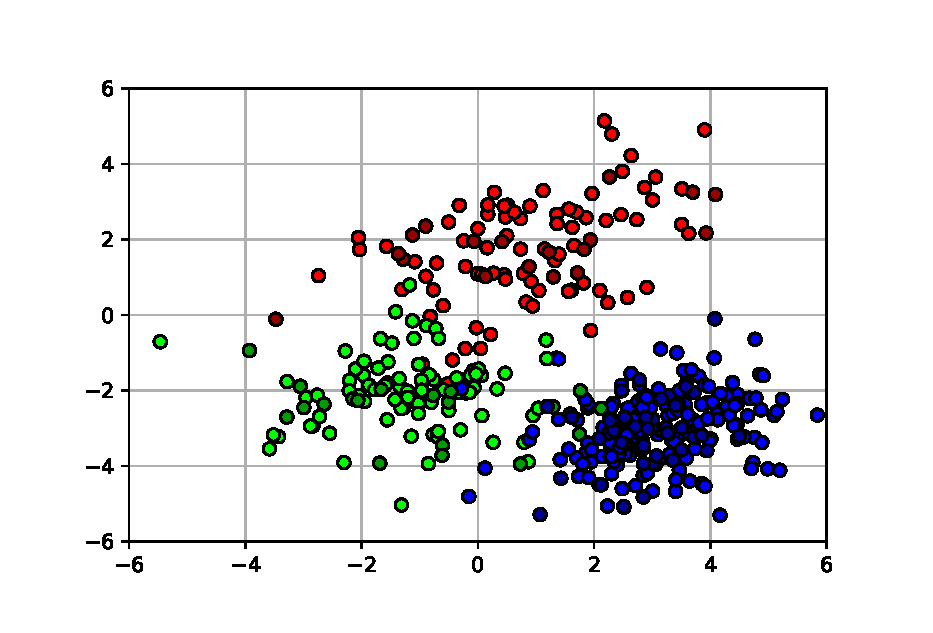
\includegraphics[scale=.65,trim=35 20 35 25]{Drawings/data.eps}}
      \caption{Generated data with the parameter specification of Eq. \ref{eq:means}, and Eq. \ref{eq:CVMatrices}. The blue group
      corresponds to $\mu_{1}$, $\Sigma_{1}$, the red group corresponds to  $\mu_{2}$, $\Sigma_{2}$, and the green group corresponds to  $\mu_{3}$, $\Sigma_{3}$.}
      \label{fig:data}
\end{figure}

\subsection{EM Algorithm}
\label{sec:Experiment_EM_Algorithm}

The execution of the expectation maximization algorithm with with Gaussian mixtures is presented in Fig.~\ref{fig:GMMIteration1}, Fig.~\ref{fig:GMMIteration7}, Fig.~\ref{fig:GMMIteration14}, and  Fig.~\ref{fig:GMMIteration20}. The initialization values for the means were $\mu_{1} = [-2 \quad 5] ^T$, $\mu_{2} = [0.1 \quad 4.5] ^T$, and $\mu_{3} = [4.2 \quad 0.2] ^T$ and the covariance matrices $\Sigma_{k}$ were initialized as identity matrices.  In order to avoid cluttering the images with too many level curves, we decided to plot level curves from $L = 0.001$ to $L = 0.019$ in increments of $0.001$. The trajectory of the means as the algorithm evolves in time is presented in Fig.~\ref{fig:ui_Paths_GMM}.

 Note that in the first iteration, Fig.~\ref{fig:GMMIteration1}, $\mu_{2}$ and $\mu_{3}$ are set relatively close that the maximum level curve sets the two groups as
 one; but as the computation is carried out,Fig.~\ref{fig:GMMIteration7}, the curve of the maximum level begins to split. At the $14^{th}$ iteration we can see three closed curves appear. At the end, in Fig.~\ref{fig:GMMIteration20} we can see there is not a major change on the form of the closed curves. Also note that the maximum level curves are getting stretch as the algorithm progresses, giving account of the modification of the covariance matrices.
 
\begin{figure}[ht!]
 \begin{center}
  	\subfigure[\label{fig:GMMIteration1}]{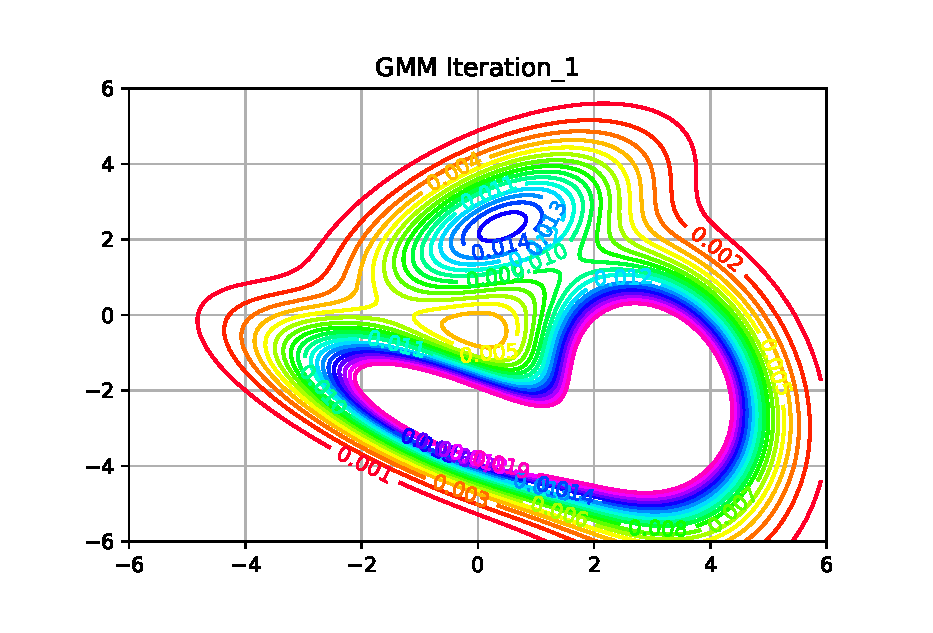
\includegraphics[width=0.36\textwidth,trim=35 20 35 25]{Drawings/GMMIteration1.eps}}
 	\subfigure[\label{fig:GMMIteration7}]{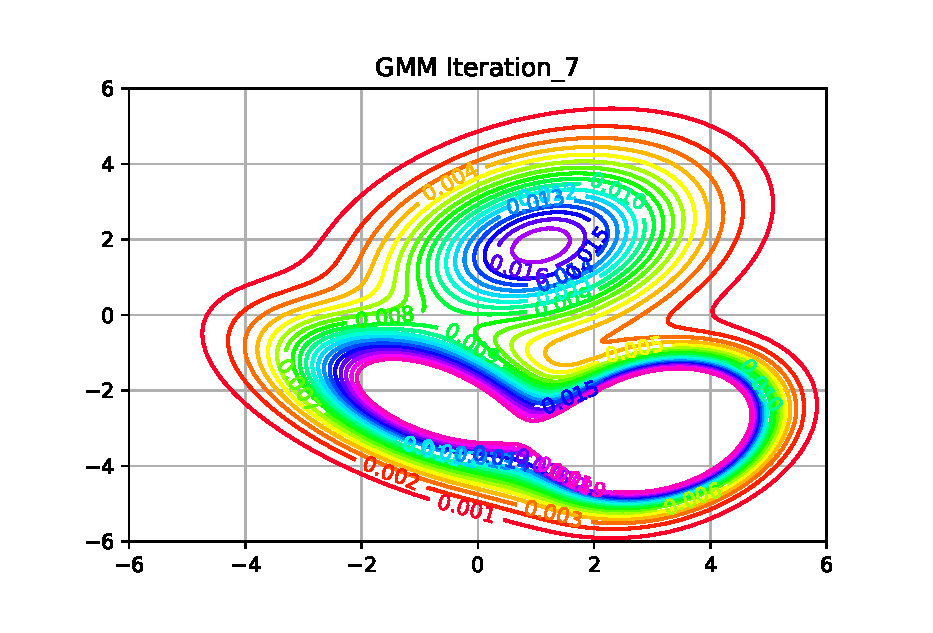
\includegraphics[width=0.36\textwidth,trim=35 20 35 5]{Drawings/GMMIteration7.eps}}
 	\subfigure[\label{fig:GMMIteration14}]{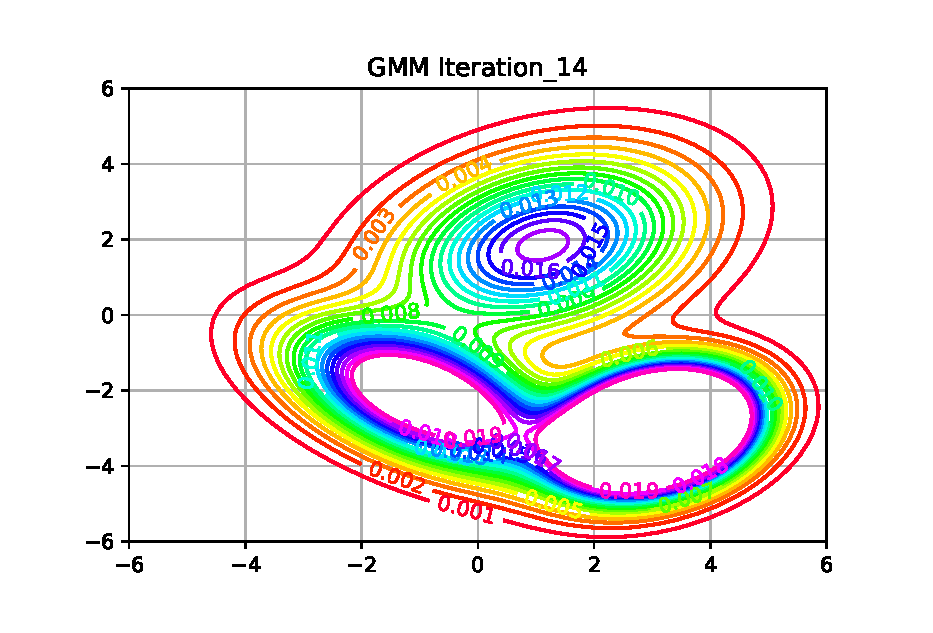
\includegraphics[width=0.36\textwidth,trim=35 20 35 5]{Drawings/GMMIteration14.eps}}
 	\subfigure[\label{fig:GMMIteration20}]{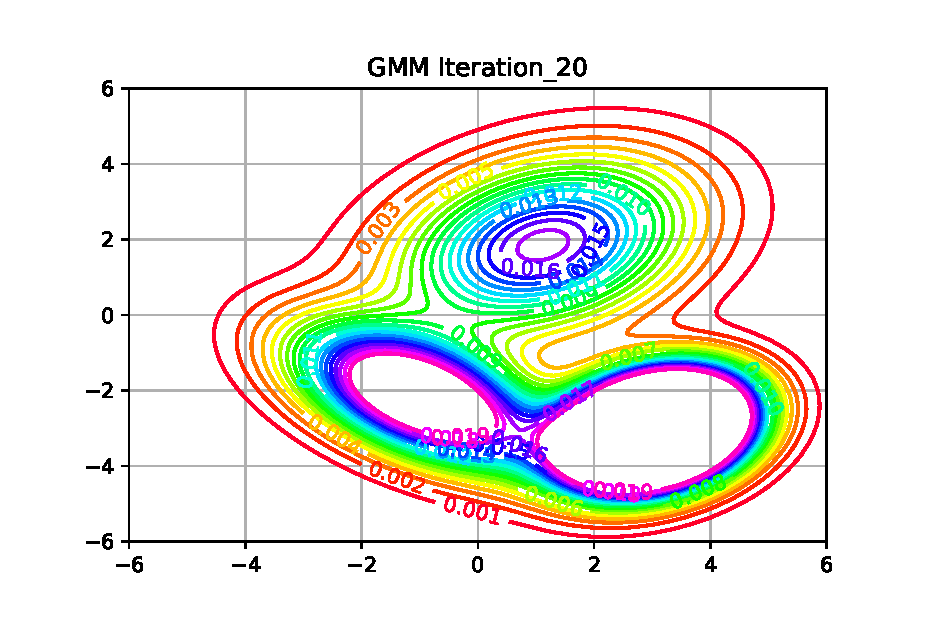
\includegraphics[width=0.36\textwidth,trim=35 20 35 5]{Drawings/GMMIteration20.eps}}
         \caption{Evolution of the Expectation Maximization algorithm using Gaussian mixture models at iterations (a) $1$, (b) $7$, (c) $14$, and (d) $20$. }
 \end{center}
\end{figure}

\subsection{Representation of the Data Likelihood}
\label{sec:Experiment_Representation_Data_Likelihood}

The log-likelihood is presented in Eq. \ref{eq:loglikelihood} and the evolution of this measure is depicted on Fig.\ref{fig:loglikelihookGMM}. As the algorithm 
finds the means, covariance matrices and posterior probabilities based on the maximization of the log-likelihood, the best stopping criterion should be to
halt the iterations when we perceive a decrement in the log-likelihood quantity.

However, note that Eq. \ref{eq:loglikelihood} requires the computation with all the samples $M$, over the number of latent variables $N$, which is $O(NM)$. 
Note that in Fig.~\ref{fig:ui_Paths_GMM} we can see that after the first iteration, the means have very small displacements, which hints that a more appropriate stopping criterion could be the Euclidean norm of the means' displacements. The displacements of the means and the norm of the displacements as the  expectation maximization algorithm with with Gaussian mixtures evolves is presented in Fig.~\ref{fig:EvolutionMuDisplacement_GMM}. Note that the norm bounds the displacements of the means, guaranteeing that all the displacement are below or equal the stopping value assigned to the norm. In our case, we took a very
conservative approach and required the norm of the displacements to be $0.01$

\subsection{Unsupervised Classification}
\label{sec:Experiment_Unsupervised_Classification}

A scatter plot of the data is depicted in Fig.~\ref{fig:ScatterPlot}, where we assigned the final iteration of Eq. \ref{eq:GMMEq} to the size of the ball of each 
sample.

\begin{figure}[thpb]
      \centering
      \framebox{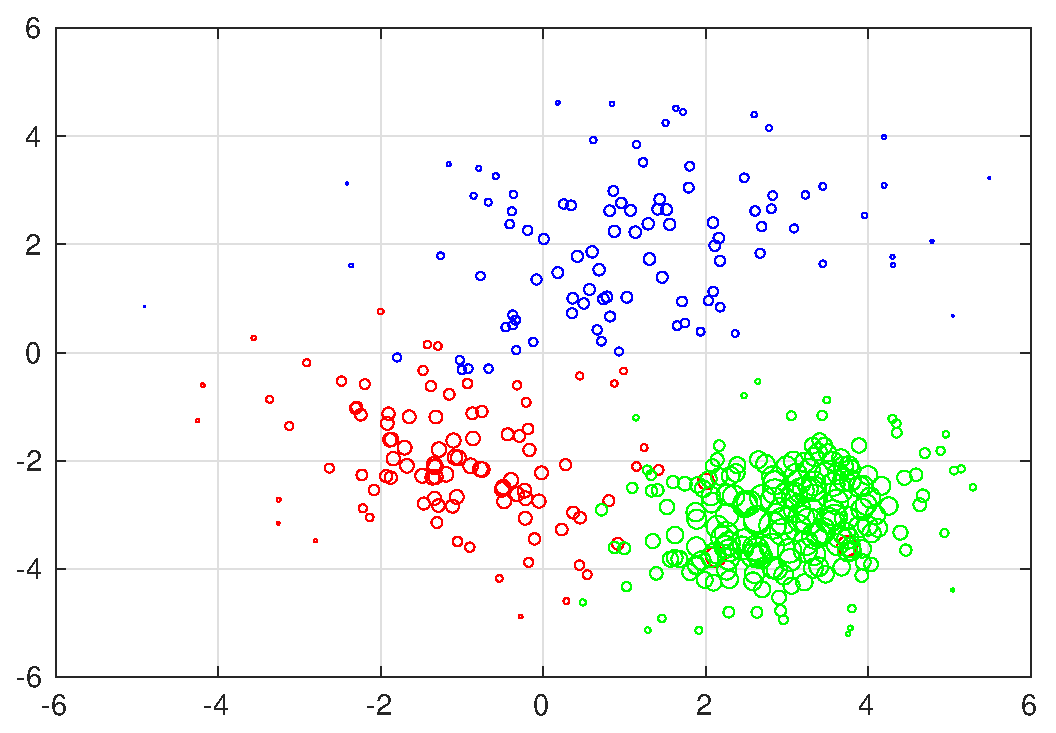
\includegraphics[scale=.45]{Drawings/ScatterPlot.eps}}
      \caption{Scatter plot. The bigger the balls are, the higher the probability value the samples have assigned to them.}
      \label{fig:ScatterPlot}
\end{figure}

A classification scheme based on the GMM model would be to take each Gaussian that makes part of Eq. \ref{eq:GMMEq} and assign a threshold $\epsilon_{k}$ on each function.  Then, a sample $x_{n}$ belongs to a feature $k$ if  
\begin{equation*}
    \pi_{k} \mathcal{N}(x | \mu_{k},\Sigma_{k}) > \epsilon_{k}.
\end{equation*}

A representation of the classification parameters explained before is depicted on Fig.~\ref{fig:LevelsClassificationInsight}, where the level curves with $L = \epsilon_{k}$ are calculated for each $\pi_{k} \mathcal{N}(x | \mu_{k},\Sigma_{k}) $.

\begin{figure}[thpb]
      \centering
      \framebox{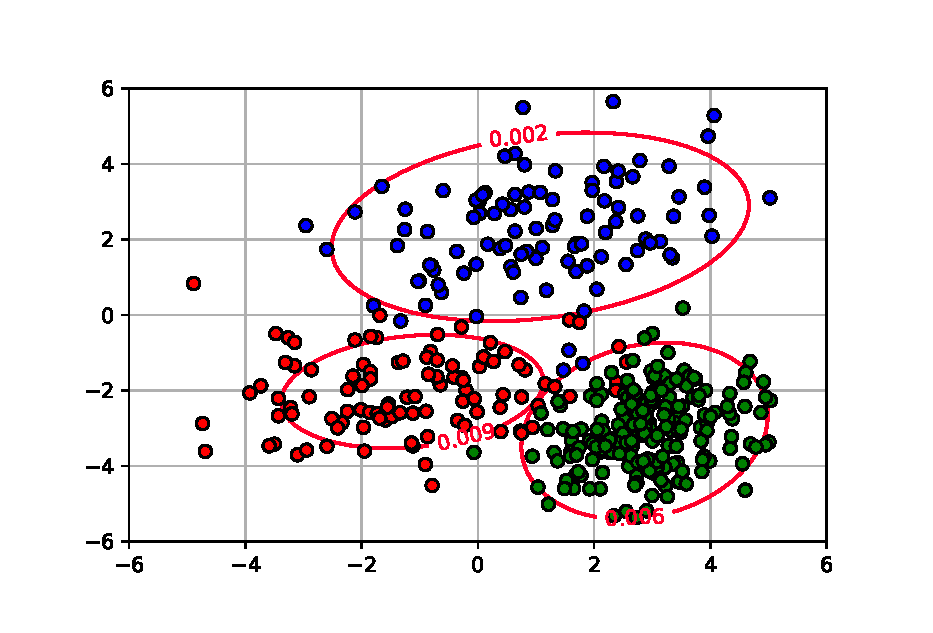
\includegraphics[scale=.65,trim=25 20 35 25]{Drawings/LevelsClassificationInsight.eps}}
      \caption{Classification scheme. In this case, $\epsilon_{blue} = 0.004$, $\epsilon_{red} = 0.012$, and $\epsilon_{green} = 0.006$}.
      \label{fig:LevelsClassificationInsight}
\end{figure}

\subsection{Comparison to the K-means Algorithm}
\label{sec:Experiment_Comparison_Kmeans_Algorithm}

The other approach available for unsupervised classifications is k-means. We are taking the same artificial data depicted in Fig.~\ref{eq:CVMatrices} as
input for our implementation of k-means.


\subsubsection{Mahalanobis distance}
\label{sec:Experiment_Mahalanobis_distance}

A positive-definite matrix $A$ can generate a norm of the form $\sqrt{x^{T}Ax}$. Although the covariance matrices $\Sigma_{k}$ are only positive-semidefinite 
matrices, a norm that takes into account the correlation among the samples in a problem of classification is very helpful. Instead of using the euclidean norm on 
function $\gamma(z_{nk})$ for the k-means procedure, we use the Mahalanobis distance which is defined as

\begin{equation*}
 d_{\Sigma_{k}} = \sqrt{(x_{n} - \mu_{k})^{T}\Sigma_{k} (x_{n} - \mu_{k})},
\end{equation*}

\subsubsection{K-means procedure and Parameter update}
\label{sec:Experiment_Kmeans_procedure}

 The initialization values for the means were $\mu_{1} = [ -0.76 \quad -2.16] ^T$, $\mu_{2} = [3.40  \quad -3.38] ^T$, and $\mu_{3} = [3.33 \quad -2.53] ^T$ and the covariance matrices $\Sigma_{k}$ were initialized as identity matrices. The trajectory of the means as the algorithm evolves in time is presented in Fig.~\ref{fig:ui_Paths_K_MEANS}.
\begin{figure}[ht!]
 \begin{center}
  	\subfigure[\label{fig:KMeansIteration1}]{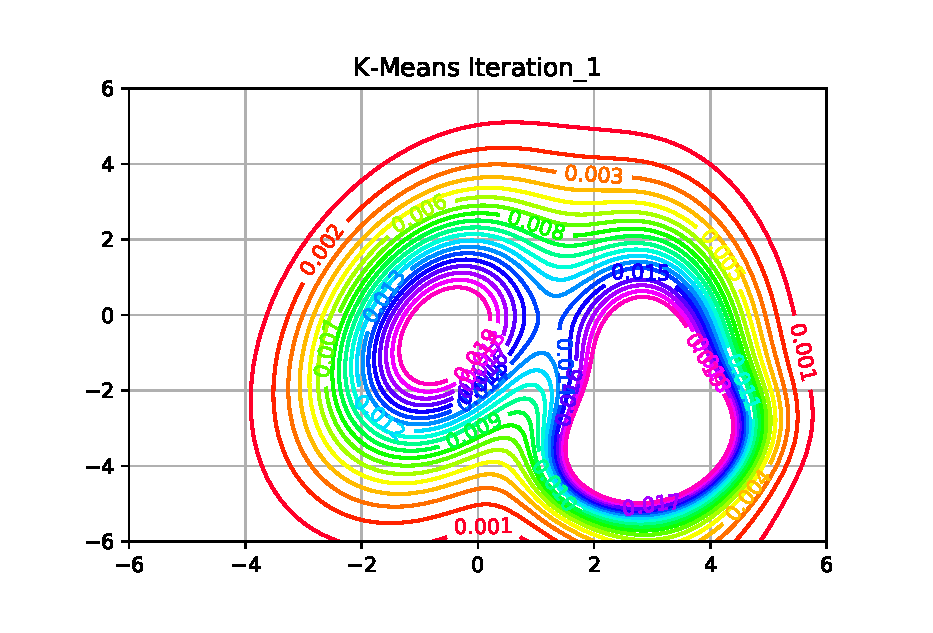
\includegraphics[width=0.36\textwidth,trim=35 20 35 25]{Drawings/KMeansIteration1.eps}}
  	\subfigure[\label{fig:KMeansIteration23}]{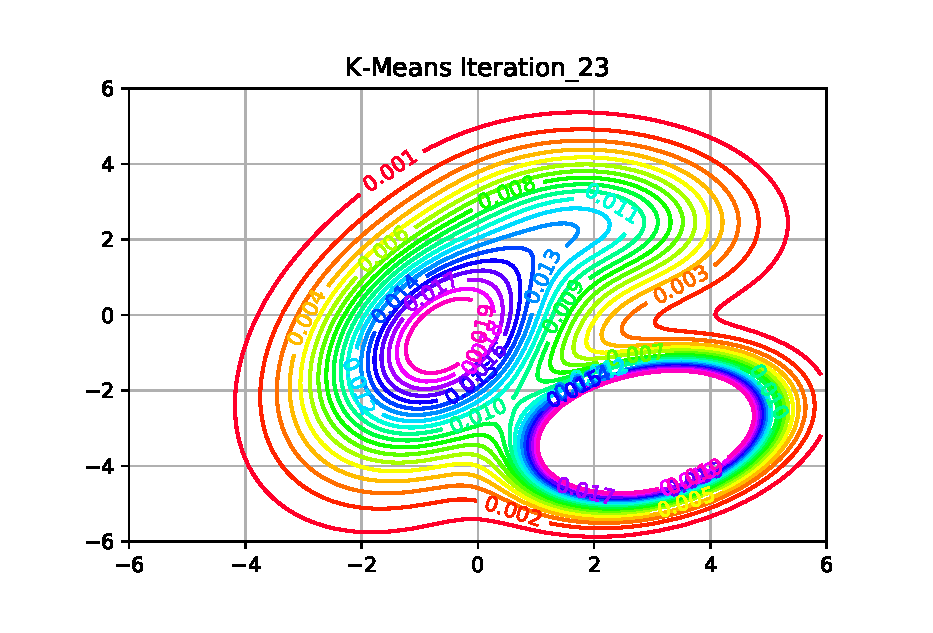
\includegraphics[width=0.36\textwidth,trim=35 20 35 5]{Drawings/KMeansIteration23.eps}}
  	\subfigure[\label{fig:KMeansIteration38}]{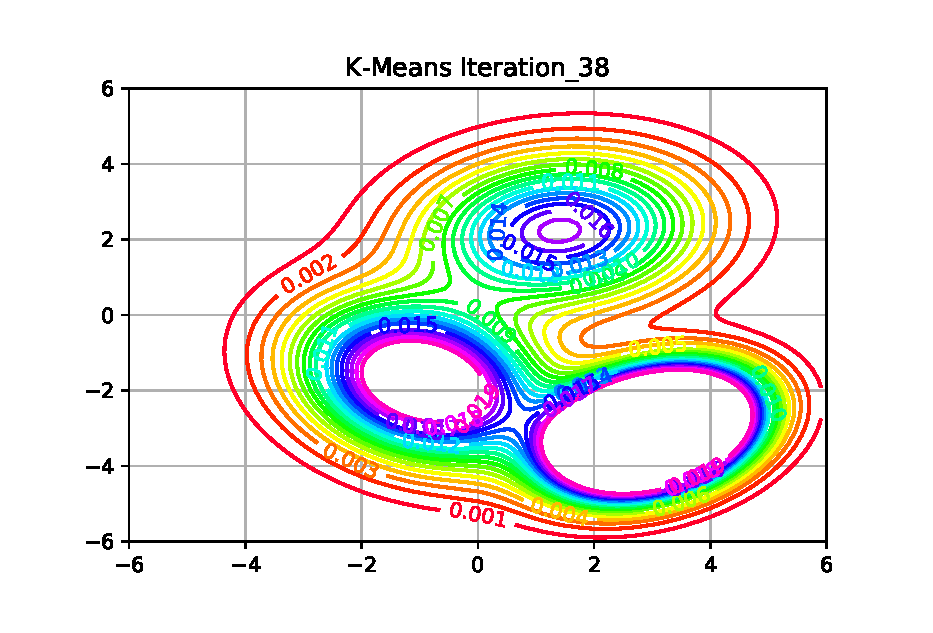
\includegraphics[width=0.36\textwidth,trim=35 20 35 5]{Drawings/KMeansIteration38.eps}}
  	\subfigure[\label{fig:KMeansIteration53}]{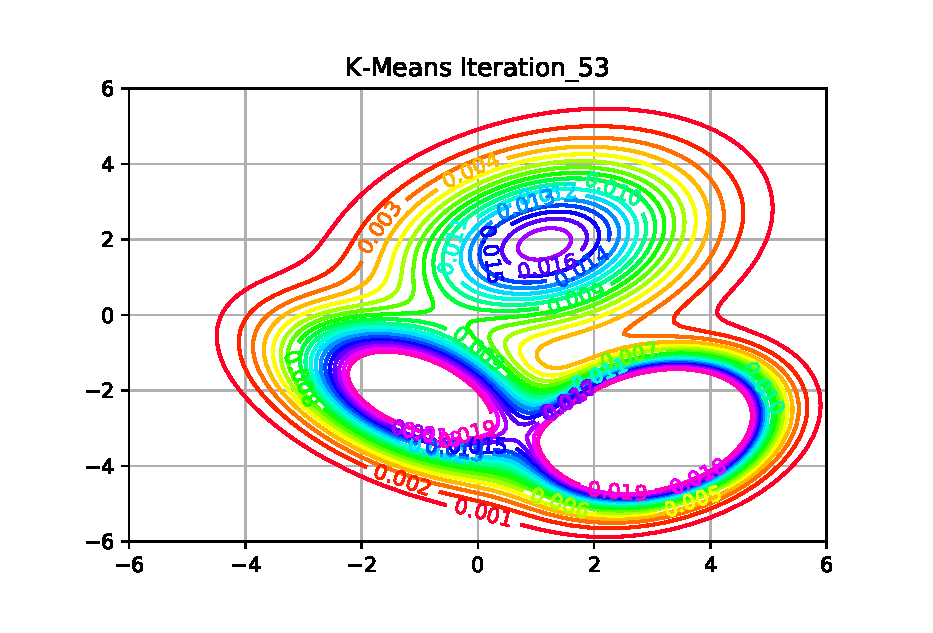
\includegraphics[width=0.36\textwidth,trim=35 20 35 5]{Drawings/KMeansIteration53.eps}}
         \caption{Output of \emph{svmtrain} with different values of $\sigma$. (a), $\sigma = 0.05$. (b), $\sigma = 1$. (c), $\sigma = 1.4$.}
 \end{center}
\end{figure}

Because means $\mu_{1}$ and $\mu_{3}$ are very close to the mean of the group of green markers, the first iteration shown in Fig.~\ref{fig:KMeansIteration1} suggest there are going to be two groups. Note that in this case Fig.~\ref{fig:ui_Paths_K_MEANS} shows that the displacements of the means is reduced compared to how the means moved on the Gaussian mixture model, therefore for this particular choice of initial means the algorithm is going to take longer to converge to our stopping criterion. As the algorithm progresses and  Fig.~\ref{fig:ui_Paths_K_MEANS} shows, $\mu_{1}$ starts moving to the top of the space starting to create a closed curve around it, as shown in  Fig.~\ref{fig:KMeansIteration23}. By the $38^{th}$ the three groups are clearly defined and in Fig.~\ref{fig:KMeansIteration53} we can see that the covariance matrices have influenced the closed curves by elongating the groups at the bottom of the graph. We confronted the Log-likelihood for  Expectation Maximization with Gaussian mixture models in both the train set and the test set: while the  Log-likelihood for the train data in monotonically increasing, the Log-likelihood for the test data has a maximum. That is the stopping criterion: the maximum of the Log-likelihood for the test data .

\begin{figure*}[ht!]
 \begin{center}
  	\subfigure[\label{fig:ui_Paths_GMM}]{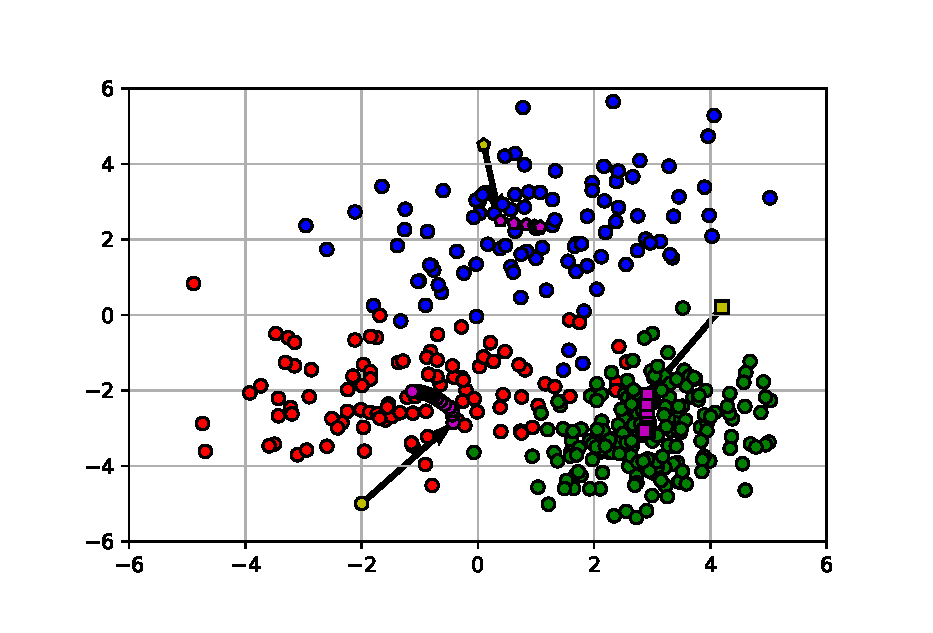
\includegraphics[width=0.4\textwidth,trim=35 20 35 25]{Drawings/ui_Paths_GMM.eps}}\hfill
 	\subfigure[\label{fig:ui_Paths_K_MEANS}]{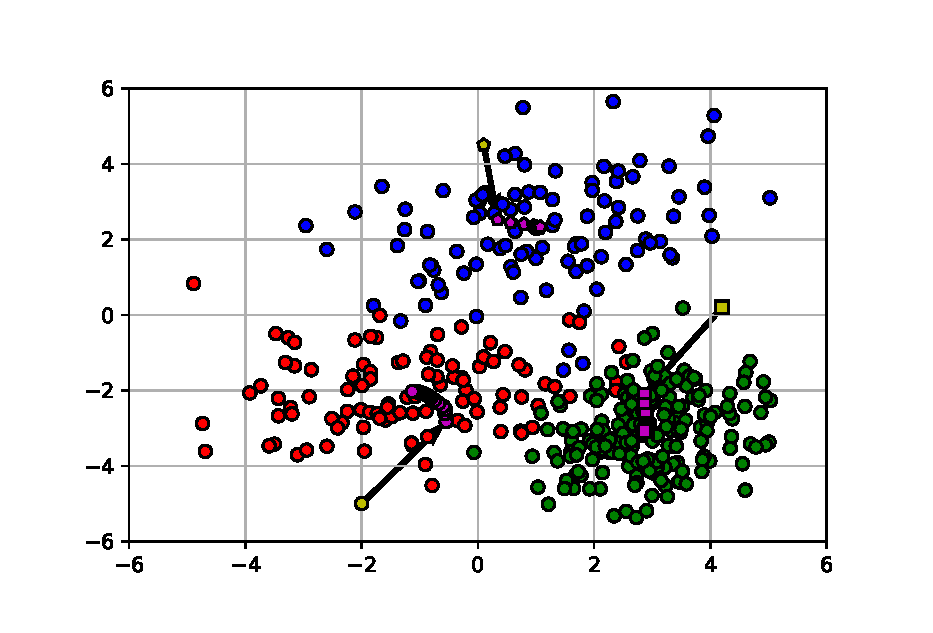
\includegraphics[width=0.4\textwidth,trim=35 20 35 25]{Drawings/ui_Paths_K_MEANS.eps}}\hfill
 	\subfigure[\label{fig:EvolutionMuDisplacement_GMM}]{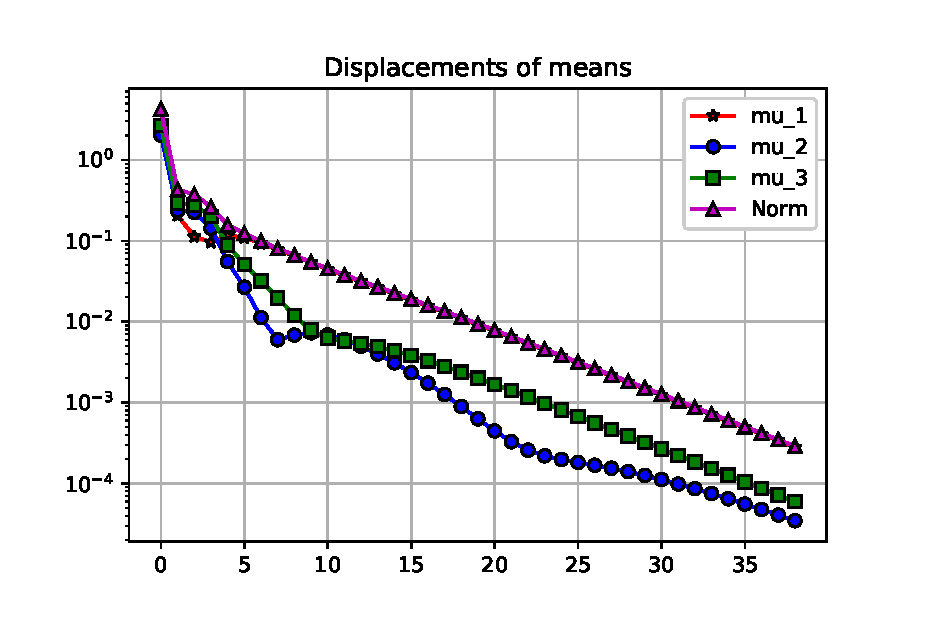
\includegraphics[width=0.4\textwidth,trim=35 20 35 5]{Drawings/EvolutionMuDisplacement_GMM.eps}}\hfill
 	\subfigure[\label{fig:EvolutionMuDisplacement_K_MEANS}]{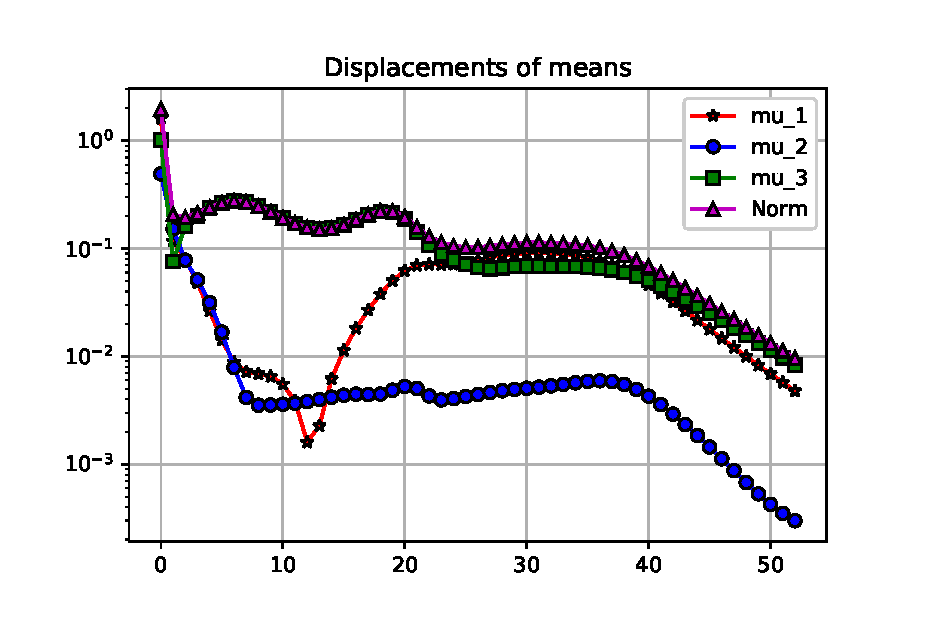
\includegraphics[width=0.4\textwidth,trim=35 20 35 5]{Drawings/EvolutionMuDisplacement_K_MEANS.eps}}\hfill
 	\subfigure[\label{fig:loglikelihookGMMTheOne}]{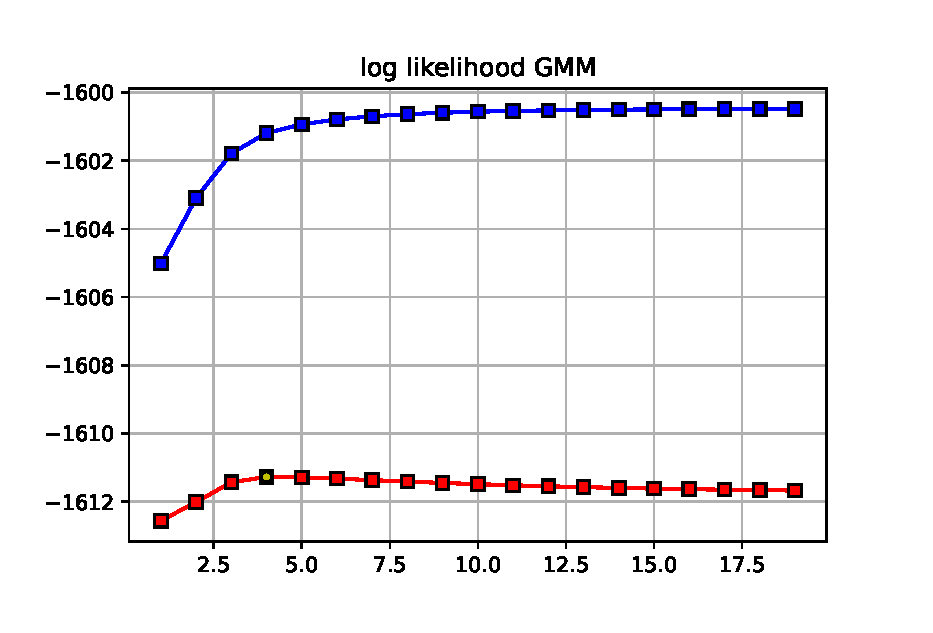
\includegraphics[width=0.4\textwidth,trim=35 20 35 5]{Drawings/loglikelihookGMMTheOne.eps}}\hfill
  \caption{Comparison between Expectation Maximization with Gaussian mixture models and k-means. (a) Trajectory of the means, and (c) displacement of means for  Expectation Maximization with Gaussian mixture models. (b) Trajectory of the means,, and (e) displacement of means for k-means. (e) Log-likelihood for Expectation Maximization with Gaussian mixture models}
 \end{center}
\end{figure*}

\subsubsection{Parameter initialization, growing-pruning and use in an 10
dimensional problem}
\label{sec:Experiment_growing_pruning_10}

The parameter initialization goes as follows:

\begin{enumerate}
\item Start by choosing a sample randomly from the set of samples. As it is assumed that the distribution of the clusters inside the set of samples is Gaussian, there is
about a $65$ \% change the sample is close to the actual mean of a cluster withing a standard deviation distance.
\item Compute the distance between your selected sample and the rest of the samples and sort them into increasing order.
\item Assign a probability to each distance according to 
\begin{equation*}
   \mathbb{P}(x_{i}) = \frac{d_{i}}{\sum_{j}d_{j}}.
\end{equation*}
\item Select your initial mean in regions of the probability you just assigned where the slope is not pronounced. 
\end{enumerate}

Consider Fig.~\ref{fig:ProbabilityAssigment}. The red dots indicate the samples where the slope of the probability function assigned to the distance changes dramatically. In the regions between them the slope is kept constant, suggesting a cluster. Therefore the selection of the initial means should be samples of these regions.

\begin{figure}[thpb]
      \centering
      \framebox{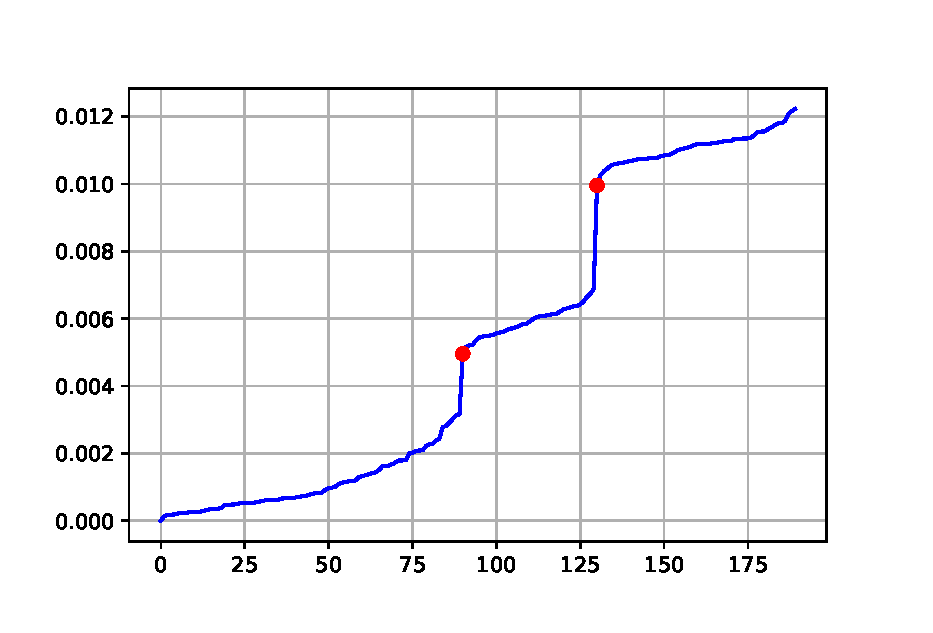
\includegraphics[scale=.65,trim=20 20 35 25]{Drawings/ProbabilityAssigment.eps}}
      \caption{Selection of initial means. }
      \label{fig:ProbabilityAssigment}
\end{figure}

In contrast to this activity where we fabricated the sample data, we don't know how many clusters are present in the sample set. Therefore we can assign more clusters than necessary or less. If we assign more clusters than required, some means are going to converge to the same target mean while having similar covariance matrices, then it is necessary to do \emph{pruning}, that is, compute a single center with the average of the converging means and their respective covariance matrices. On the other hand, if the ratio of the singular values of the covariance matrix is very high, we split the mean into the direction related to the highest singular value, this is known as \emph{growing}.


%%%%%%%%%%%%%%%%%%%%%%%%%%%%%%%%%%%%%%%%%%%%%%%%%%%%%%%%%%%%%%%%%%%%%%%%%%%%%%%%

\section{Conclusion}
\label{sec:Conclusion}

The stopping criterion: because we are calculating the maximum of an increasing function such as the log-likelihood which argument is a Gaussian distribution, we
are driven into the direction of stopping the algorithm when the log-likelihood stops increasing. However, a computation with all the samples over all the assigned
latent variables makes it expensive, which lead us to use the Euclidean norm of the displacements. We selected a very conservative stopping value, which was reflected in the increased number of iterations.

Despite the fact the means $\mu_{1}$ and $\mu_{3}$ were very close to the mean of the generated green group on the k-means execution, the algorithm managed
to steer $\mu_{1}$ to create a new cluster, $\mu_{1}$ did not get stuck on the group three.  

Even though we are maximizing Eq. \ref{eq:GMMEq}, we chose its individual components as the requested classifier of Section \ref{sec:Experiment_Unsupervised_Classification}. The idea behind that decision is that Eq. \ref{eq:GMMEq} is seen as a linear
combination of Gaussian distributions, where the Gaussian distributions are thought of linearly independent functions.


 
% \subsection{SVM for Regression}
%\label{sec:ConclusionSVMRegression}


%%%%%%%%%%%%%%%%%%%%%%%%%%%%%%%%%%%%%%%%%%%%%%%%%%%%%%%%%%%%%%%%%%%%%%%%%%%%%%%%

%References are important to the reader; therefore, each citation must be complete and correct. If at all possible, references should be commonly available publications.


%\pagebreak

\bibliographystyle{IEEEtran}
\bibliography{References}

%%%%%% APPENDIX %%%%%%%
%q\input{Appendix}
\end{document}
